\documentclass[titlepage]{article}
\usepackage[margin=0.5in]{geometry}
\usepackage{graphicx}
\usepackage{minted}

\title{VLSI \\Assignment 3}
\author{Priyank Lohariwal\\BCSE IV\\Roll-001710501055}
\date{}

\begin{document}
    {\maketitle}

    \section{Describtion}
    \begin{itemize}
        \item Design a 1x2 decoder
        \begin{itemize}
            \item using gate level modelling
            \item using behavioral modelling
            \begin{itemize}
                \item using if else statement
                \item using case statement
                \item using when else statement
                \item using select when statement
            \end{itemize}
        \end{itemize}
        \item Design a 2x4 decoder 
        \begin{itemize}
            \item using gate level modelling
            \item using behavioral modelling
            \begin{itemize}
                \item using if else statement
                \item using case statement
                \item using when else statement
                \item using select when statement
            \end{itemize}
        \end{itemize}
        \item Design a 3x8 decoder
        \begin{itemize}
            \item using gate level modelling
            \item using behavioral modelling
            \begin{itemize}
                \item using if else statement
                \item using case statement
                \item using when else statement
                \item using select when statement
            \end{itemize}
        \end{itemize}
        \item Design a 3x8 decoder using 2x4 decoder and 1x2 decoder by component instantiation
        \item Design a 4x16 decoder using 2x4 decoder only by component instantiation
    \end{itemize}

    \section{Block Diagram} 
    \begin{figure}[!ht]
        \centering
        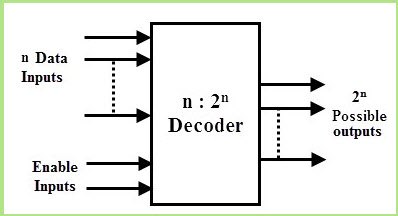
\includegraphics{./figures/Decoder-Block-Diagram.jpg}
        \caption{Decoder block diagram}
    \end{figure}

    \section{1x2 Decoder}
    \subsection{Truth Table}
    \begin{tabular}{ | c | c | c |}
        \hline
        X & Y(1) & Y(0) \\
        \hline
        0 & 0 & 1 \\
        1 & 1 & 0 \\
        \hline
    \end{tabular}
    \subsection{Circuit Diagram}
    \begin{figure}[!ht]
        \centering
        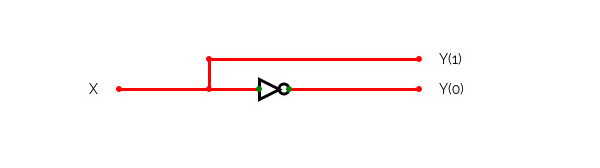
\includegraphics[width=10cm]{./figures/1x2.jpeg}
        \caption{1x2 circuit diagram}
    \end{figure}
    \subsection{Code}
    \subsubsection{Using gate level modelling}
        \inputminted{vhdl}{./codes/a3_1a.vhd}
    \subsubsection{Using if else statement} 
        \inputminted{vhdl}{./codes/a3_1ba.vhd}
    \subsubsection{Using case statement}
        \inputminted{vhdl}{./codes/a3_1bb.vhd}
    \subsubsection{Using when else statement}
        \inputminted{vhdl}{./codes/a3_1bc.vhd}
    \subsubsection{Using select when statement}
        \inputminted{vhdl}{./codes/a3_1bd.vhd}
    \subsection{Test Bench}
    \inputminted{vhdl}{./codes/tb_a3_1a.vhd}
    \subsection{Timing diagram}
    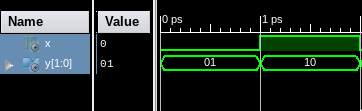
\includegraphics{./figures/td_1x2.jpeg}



%%%%%%%%%%%%%%%%%%%%%%%%%%%%%%%%%%%%%%%%%%%%%%%%%%


    \section{2x4 Decoder}
    \subsection{Truth Table}
    \begin{tabular}{| c | c | c | c | c | c |}
        \hline
        X(1) & X(0) & Y(3) & Y(2) & Y(1) & Y(0) \\
        \hline
        0 & 0 & 0 & 0 & 0 & 1 \\
        0 & 1 & 0 & 0 & 1 & 0 \\
        1 & 0 & 0 & 1 & 0 & 0 \\
        1 & 1 & 1 & 0 & 0 & 0 \\
        \hline
    \end{tabular}
    \subsection{Circuit Diagram}
    \begin{figure}[!ht]
        \centering
        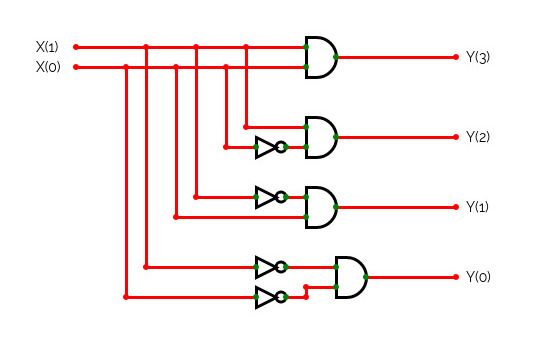
\includegraphics[width=10cm]{./figures/2x4.jpeg}
        \caption{2x4 circuit diagram}
    \end{figure}
    \subsection{Code}
    \subsubsection{Using gate level modelling}
        \inputminted{vhdl}{./codes/a3_2_1a.vhd}
    \subsubsection{Using if else statement} 
        \inputminted{vhdl}{./codes/a3_2_1ba.vhd}
    \subsubsection{Using case statement}
        \inputminted{vhdl}{./codes/a3_2_1bb.vhd}
    \subsubsection{Using when else statement}
        \inputminted{vhdl}{./codes/a3_2_1bc.vhd}
    \subsubsection{Using select when statement}
        \inputminted{vhdl}{./codes/a3_2_1bd.vhd}
    \subsection{Test Bench}
    \inputminted{vhdl}{./codes/tb_a3_2_1a.vhd}
    \subsection{Timing diagram}
    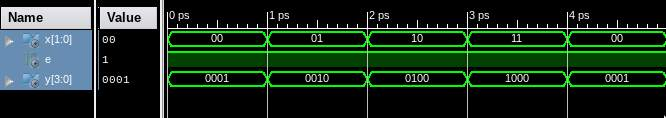
\includegraphics[width=17cm]{./figures/td_2x4.jpeg}


    \section{3x8 Decoder}
    \subsection{Truth Table}
    \begin{tabular}{| c | c | c | c | c | c | c | c | c  |c | c |}
        \hline
        X(2) & X(1) & X(0) & Y(7) & Y(6) & Y(5) & Y(4) & Y(3) & Y(2) & Y(1) & Y(0) \\
        \hline
        0 & 0 & 0 & 0 & 0 & 0 & 0 & 0 & 0 & 0 & 1 \\
        0 & 0 & 1 & 0 & 0 & 0 & 0 & 0 & 0 & 1 & 0 \\
        0 & 1 & 0 & 0 & 0 & 0 & 0 & 0 & 1 & 0 & 0 \\
        0 & 1 & 1 & 0 & 0 & 0 & 0 & 1 & 0 & 0 & 0 \\
        1 & 0 & 0 & 0 & 0 & 0 & 1 & 0 & 0 & 0 & 0 \\
        1 & 0 & 1 & 0 & 0 & 1 & 0 & 0 & 0 & 0 & 0 \\
        1 & 1 & 0 & 0 & 1 & 0 & 0 & 0 & 0 & 0 & 0 \\
        1 & 1 & 1 & 1 & 0 & 0 & 0 & 0 & 0 & 0 & 0 \\
        \hline
    \end{tabular}
    \subsection{Circuit Diagram}
    \begin{figure}[!ht]
        \centering
        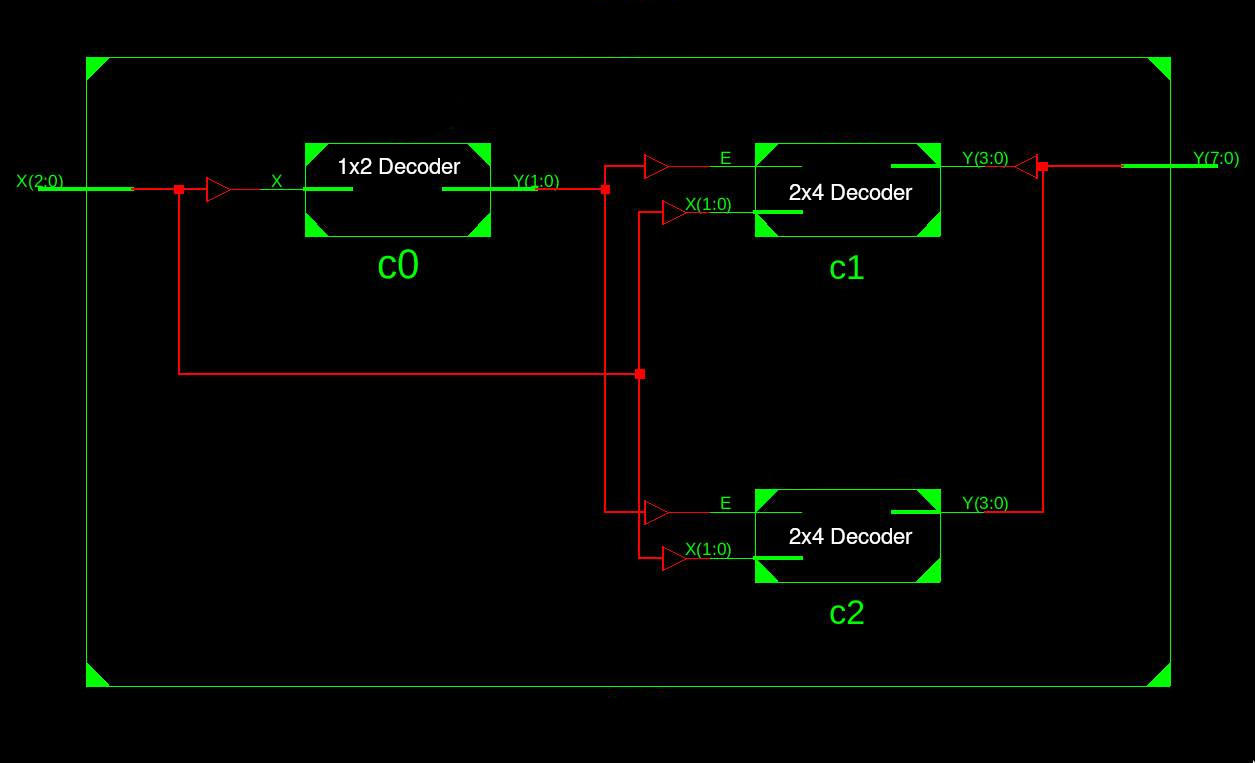
\includegraphics[width=15cm]{./figures/3x8.jpeg}
        \caption{3x8 circuit diagram}
    \end{figure}
    \subsection{Code}
    \subsubsection{Using gate level modelling}
        \inputminted{vhdl}{./codes/a3_2_2a.vhd}
    \subsubsection{Using if else statement} 
        \inputminted{vhdl}{./codes/a3_2_2ba.vhd}
    \subsubsection{Using case statement}
        \inputminted{vhdl}{./codes/a3_2_2bb.vhd}
    \subsubsection{Using when else statement}
        \inputminted{vhdl}{./codes/a3_2_2bc.vhd}
    \subsubsection{Using select when statement}
        \inputminted{vhdl}{./codes/a3_2_2bd.vhd}
    \subsubsection{Using 2x4 decoder and 1x2 decoder by component instantiation}
        \inputminted{vhdl}{./codes/a3_3.vhd}
    \subsection{Test Bench}
    \inputminted{vhdl}{./codes/tb_a3_2_2a.vhd}
    \subsection{Timing diagram}
    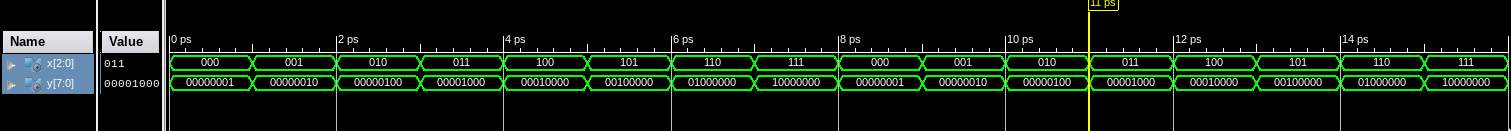
\includegraphics[width=19cm]{./figures/td_3x8.jpeg}


    \section{4x16 Decoder}
    \subsection{Truth Table}
    \begin{tabular}{| c | c |}
        \hline
        X(3 - 0) & Y(15 - 0) \\
        \hline
        0000 & 0000000000000001 \\
        0001 & 0000000000000010 \\
        0010 & 0000000000000100 \\
        0011 & 0000000000001000 \\
        0100 & 0000000000010000 \\
        0101 & 0000000000100000 \\
        0110 & 0000000001000000 \\
        0111 & 0000000010000000 \\
        1000 & 0000000100000000 \\
        1001 & 0000001000000000 \\
        1010 & 0000010000000000 \\
        1011 & 0000100000000000 \\
        1100 & 0001000000000000 \\
        1101 & 0010000000000000 \\
        1110 & 0100000000000000 \\
        1111 & 1000000000000000 \\
        \hline
    \end{tabular}
    \subsection{Circuit Diagram}
    \begin{figure}[!ht]
        \centering
        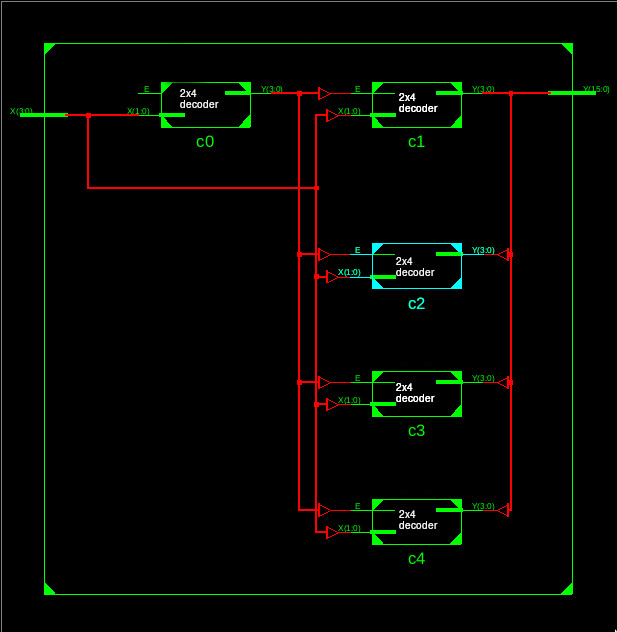
\includegraphics[width=15cm]{./figures/4x16.jpeg}
        \caption{4x16 circuit diagram}
    \end{figure}
    \subsection{Code}
    \subsubsection{Using 2x4 decoder only by component instantiation}
    \inputminted{vhdl}{./codes/a3_4.vhd}
    \subsection{Test Bench}
    \inputminted{vhdl}{./codes/tb_a3_4.vhd}
    \subsection{Timing diagram}
    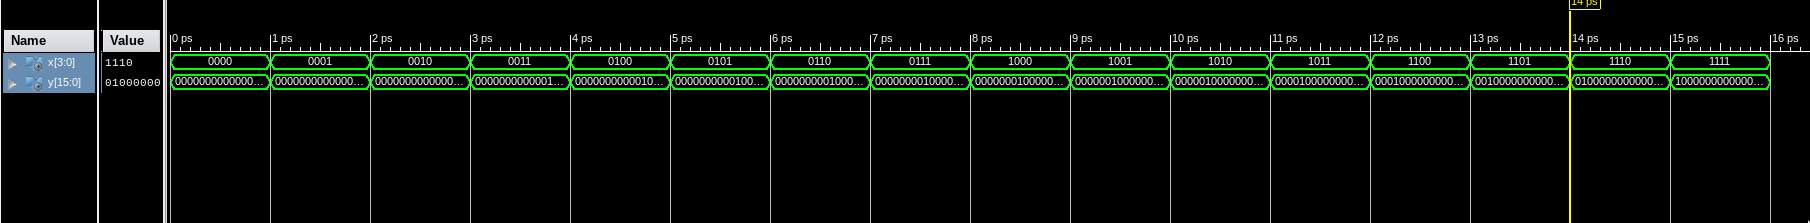
\includegraphics[width=19cm]{./figures/td_4x16.jpeg}

\end{document}
